\documentclass[a4paper,12pt]{article}
\usepackage[T2A]{fontenc}
\usepackage[utf8x]{inputenc}
\usepackage[english,russian]{babel}
\usepackage{amssymb,amsfonts,amsmath,mathtext}
\usepackage[unicode]{hyperref}
\usepackage{listings}
\usepackage{graphicx}
\usepackage{float}
\graphicspath{{images/}}
\newcommand{\anonsection}[1]{\section*{#1}\addcontentsline{toc}{section}{#1}}

\begin{document}

% Титульный лист

\begin{titlepage}
\newpage

\begin{center}

\textit{Министерство науки и высшего образования Российской Федерации \\ 
Федеральное государственное бюджетное образовательное \\
учреждение высшего образования \\
«Московский государственный технический университет \\
имени Н.Э. Баумана (национальный исследовательский университет)» \\
(МГТУ им. Н.Э. Баумана) \\}
\hrulefill
\end{center}

\vspace{2em}

\begin{flushleft}
ФАКУЛЬТЕТ <<Информатика и системы управления>> \\
\vspace{0.5em}
КАФЕДРА <<Программное обеспечение ЭВМ и информационные технологии>>
\end{flushleft}


\vspace{8em}

\begin{center}
\LARGE Лабораторная работа №3 \\
\end{center}

\vspace{1.5em}

\begin{center}
\textsc{Сортировки массивов}
\end{center}

\vspace{6em}

\begin{center}
Головнев Н.В.

\vspace{4em}

ИУ7-54Б
\end{center}

\vspace{\fill}

\begin{center}
Москва 2019
\end{center}

\end{titlepage}

\tableofcontents

% Введение

\newpage
\anonsection{ВВЕДЕНИЕ}
Алгоритмы сортировки - это простые алгоритмы упорядочивания данных, необходимые для удобного просмотра и использования данных.

\newpage
\anonsection{ПОСТАНОВКА ЗАДАЧИ}
Необходимо на выбор реализовать 3 алгоритма сортировки. Выбор средств реализации и требований под программное обеспечение также остается за разработчиком.

\newpage
\section{АНАЛИТИЧЕСКАЯ ЧАСТЬ}
\subsection{Описание алгоритмов}
\subsubsection{Сортировка пузырьком}
Алгоритм состоит из повторяющихся проходов по сортируемому массиву. За каждый проход элементы последовательно сравниваются попарно и, если порядок в паре неверный, выполняется обмен элементов. Проходы по массиву повторяются $N - 1$ раз или до тех пор, пока на очередном проходе не окажется, что обмены больше не нужны, что означает — массив отсортирован. При каждом проходе алгоритма по внутреннему циклу, очередной наибольший элемент массива ставится на своё место в конце массива рядом с предыдущим «наибольшим элементом», а наименьший элемент перемещается на одну позицию к началу массива («всплывает» до нужной позиции, как пузырёк в воде — отсюда и название алгоритма)[\ref{site:wikipedia}].

\subsubsection{Шейкерная сортировка}
Шейкер-сортировка является усовершенствованным методом пузырьковой сортировки[\ref{site:wikipedia}]. \\
Анализируя метод пузырьковой сортировки, можно отметить два обстоятельства[\ref{site:wikipedia}]:
\begin{itemize}
\item если при движении по части массива перестановки не происходят, то эта часть массива уже отсортирована и, следовательно, ее можно исключить из рассмотрения;
\item при движении от конца массива к началу минимальный элемент «всплывает» на первую позицию, а максимальный элемент сдвигается только на одну позицию вправо.
\end{itemize}
Эти две идеи приводят к модификациям в методе пузырьковой сортировки:
\begin{itemize}
\item От последней перестановки до конца (начала) массива находятся отсортированные элементы. Учитывая данный факт, просмотр осуществляется не до конца (начала) массива, а до конкретной позиции. Границы сортируемой части массива сдвигаются на 1 позицию на каждой итерации.
\item Массив просматривается поочередно справа налево и слева направо.
\item Просмотр массива осуществляется до тех пор, пока все элементы не встанут в порядке возрастания (убывания).
\item Количество просмотров элементов массива определяется моментом упорядочивания его элементов.
\end{itemize}

\subsubsection{Сортировка поиском минимума и максимума}
В чём идея сортировок выбором?
\begin{enumerate}
\item В неотсортированном подмассиве ищется локальный максимум (минимум).
\item Найденный максимум (минимум) меняется местами с последним (первым) элементом в подмассиве.
\item Если в массиве остались неотсортированные подмассивы — смотри пункт 1.
\end{enumerate}
Похожая идея используется в шейкерной сортировке, которая является вариантом пузырьковой сортировки. Проходя по неотсортированной части массива, мы кроме максимума также попутно находим и минимум. Минимум ставим на первое место, максимум на последнее. Таким образом, неотсортированная часть при каждой итерации уменьшается сразу на два элемента[\ref{site:habr}].


\newpage
\subsection{Вывод}
Аналитически 

% Конструкторская часть

\newpage
\section{КОНСТРУКТОРСКАЯ ЧАСТЬ}

\subsection{Разработка алгоритмов}
На вход у всех алгоритмов передаются в качестве параметров:
\begin{enumerate}
\item Массив;
\item Размер массива;
\end{enumerate}
Возвращаемое значение: код ошибки (0 в случае успеха, иначе отрицательное значение). \\
Побочные эффекты: массив сортируется.

\newpage
\subsection{Схемы алгоритмов}
Ниже представлены схемы алгоритмов сортировок (сортировка пузырьком, сортировка минимум/максимум, шейкерная сортировка).
\begin{figure}[H]
\center{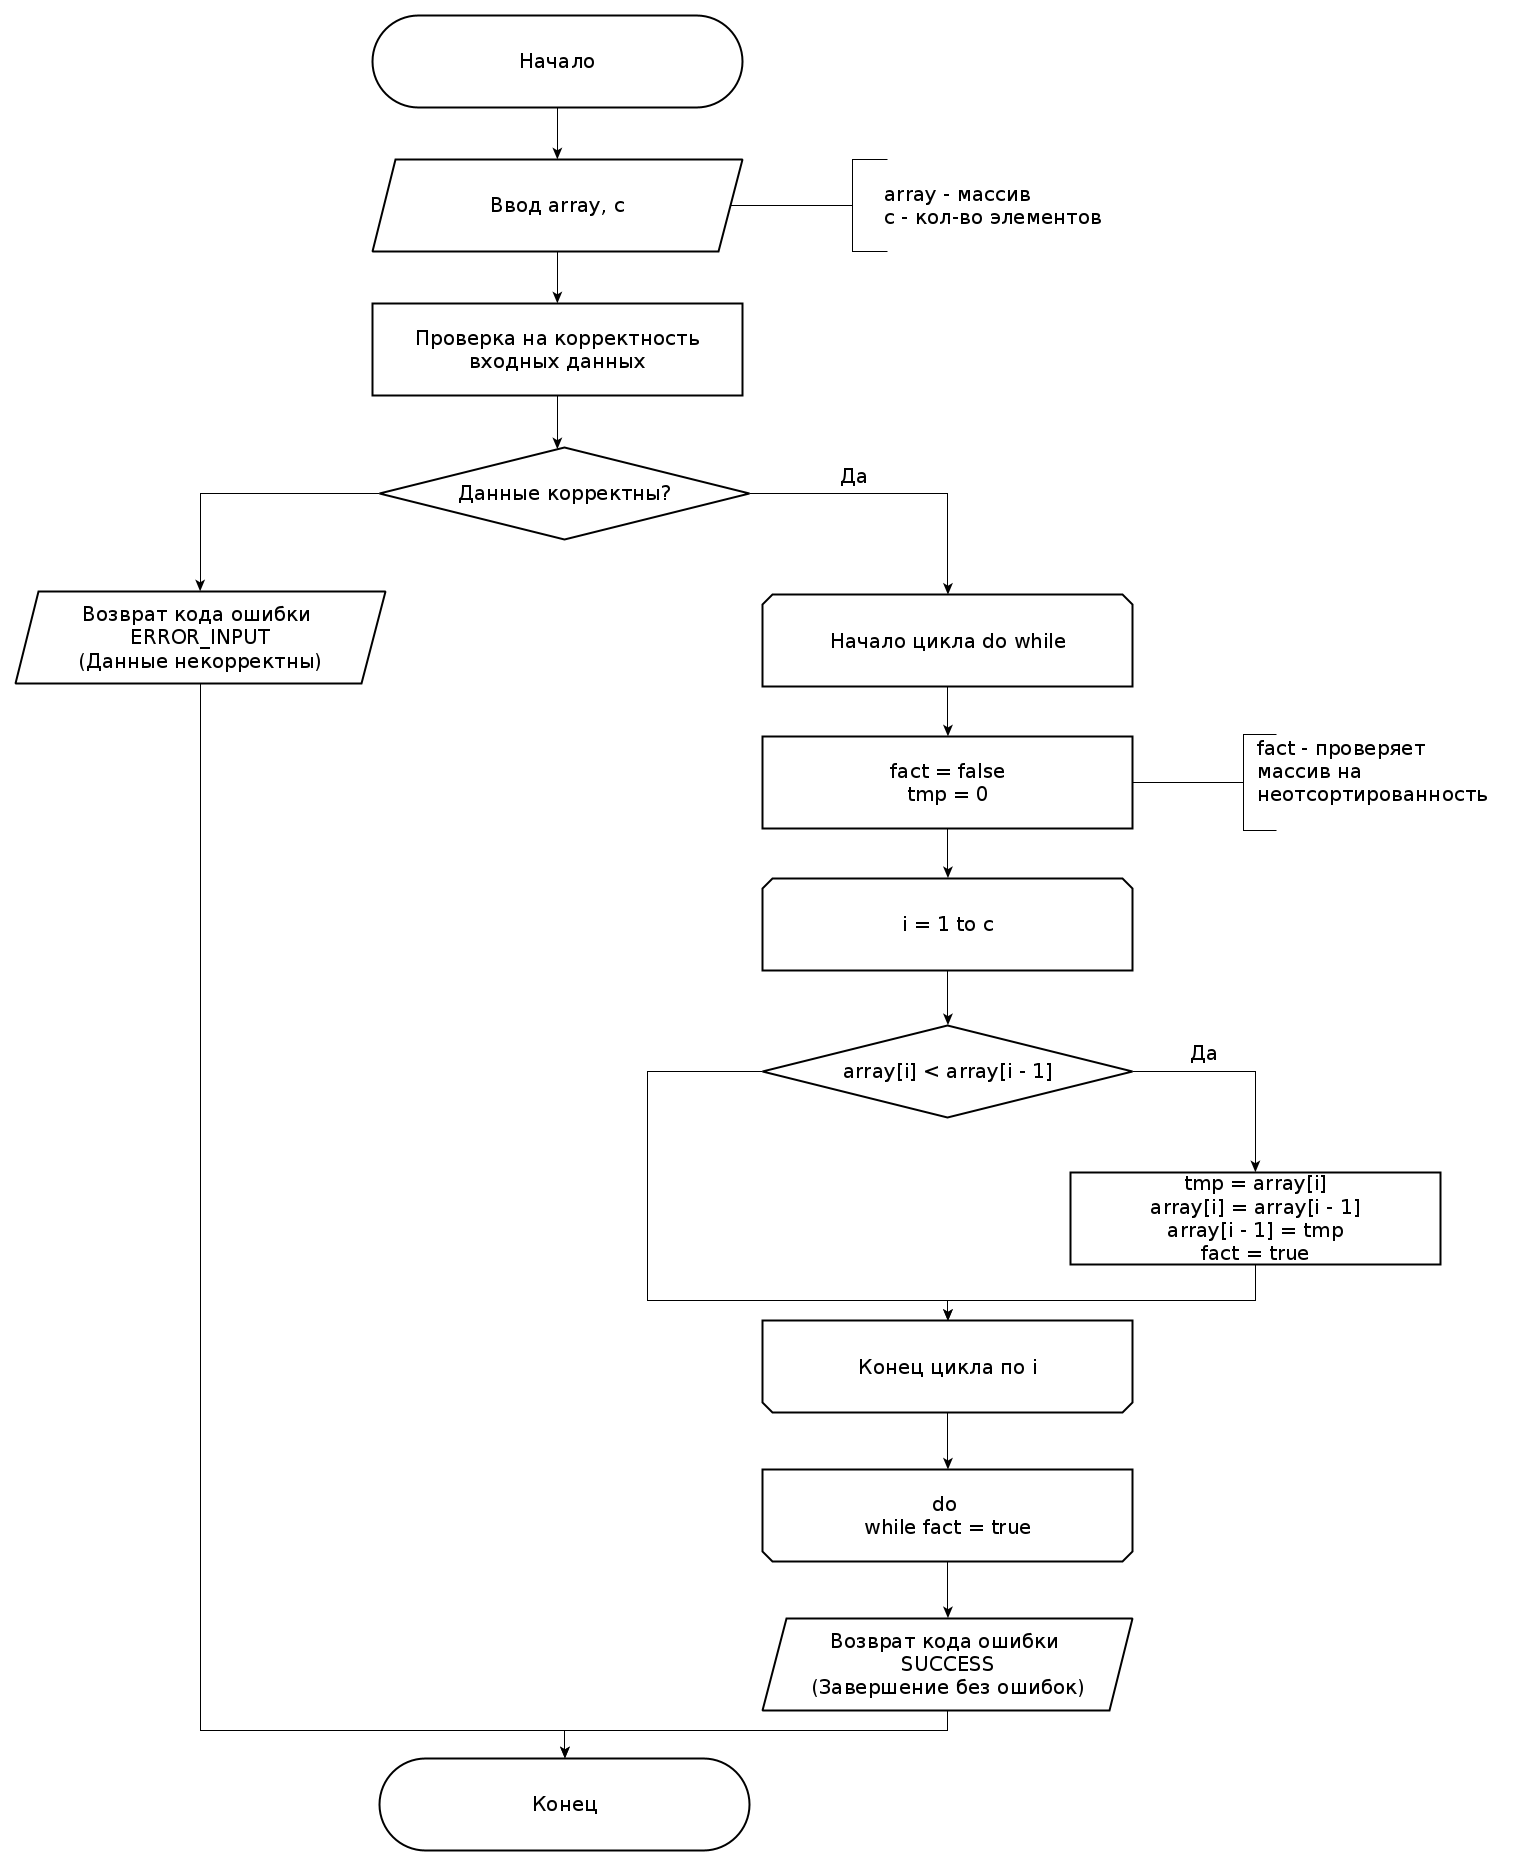
\includegraphics[scale=0.25]{sort_bubble.png}}
\caption{Схема алгоритма сортировки пузырьком}
\label{images:scheme1}
\end{figure}
\begin{figure}[p]
\center{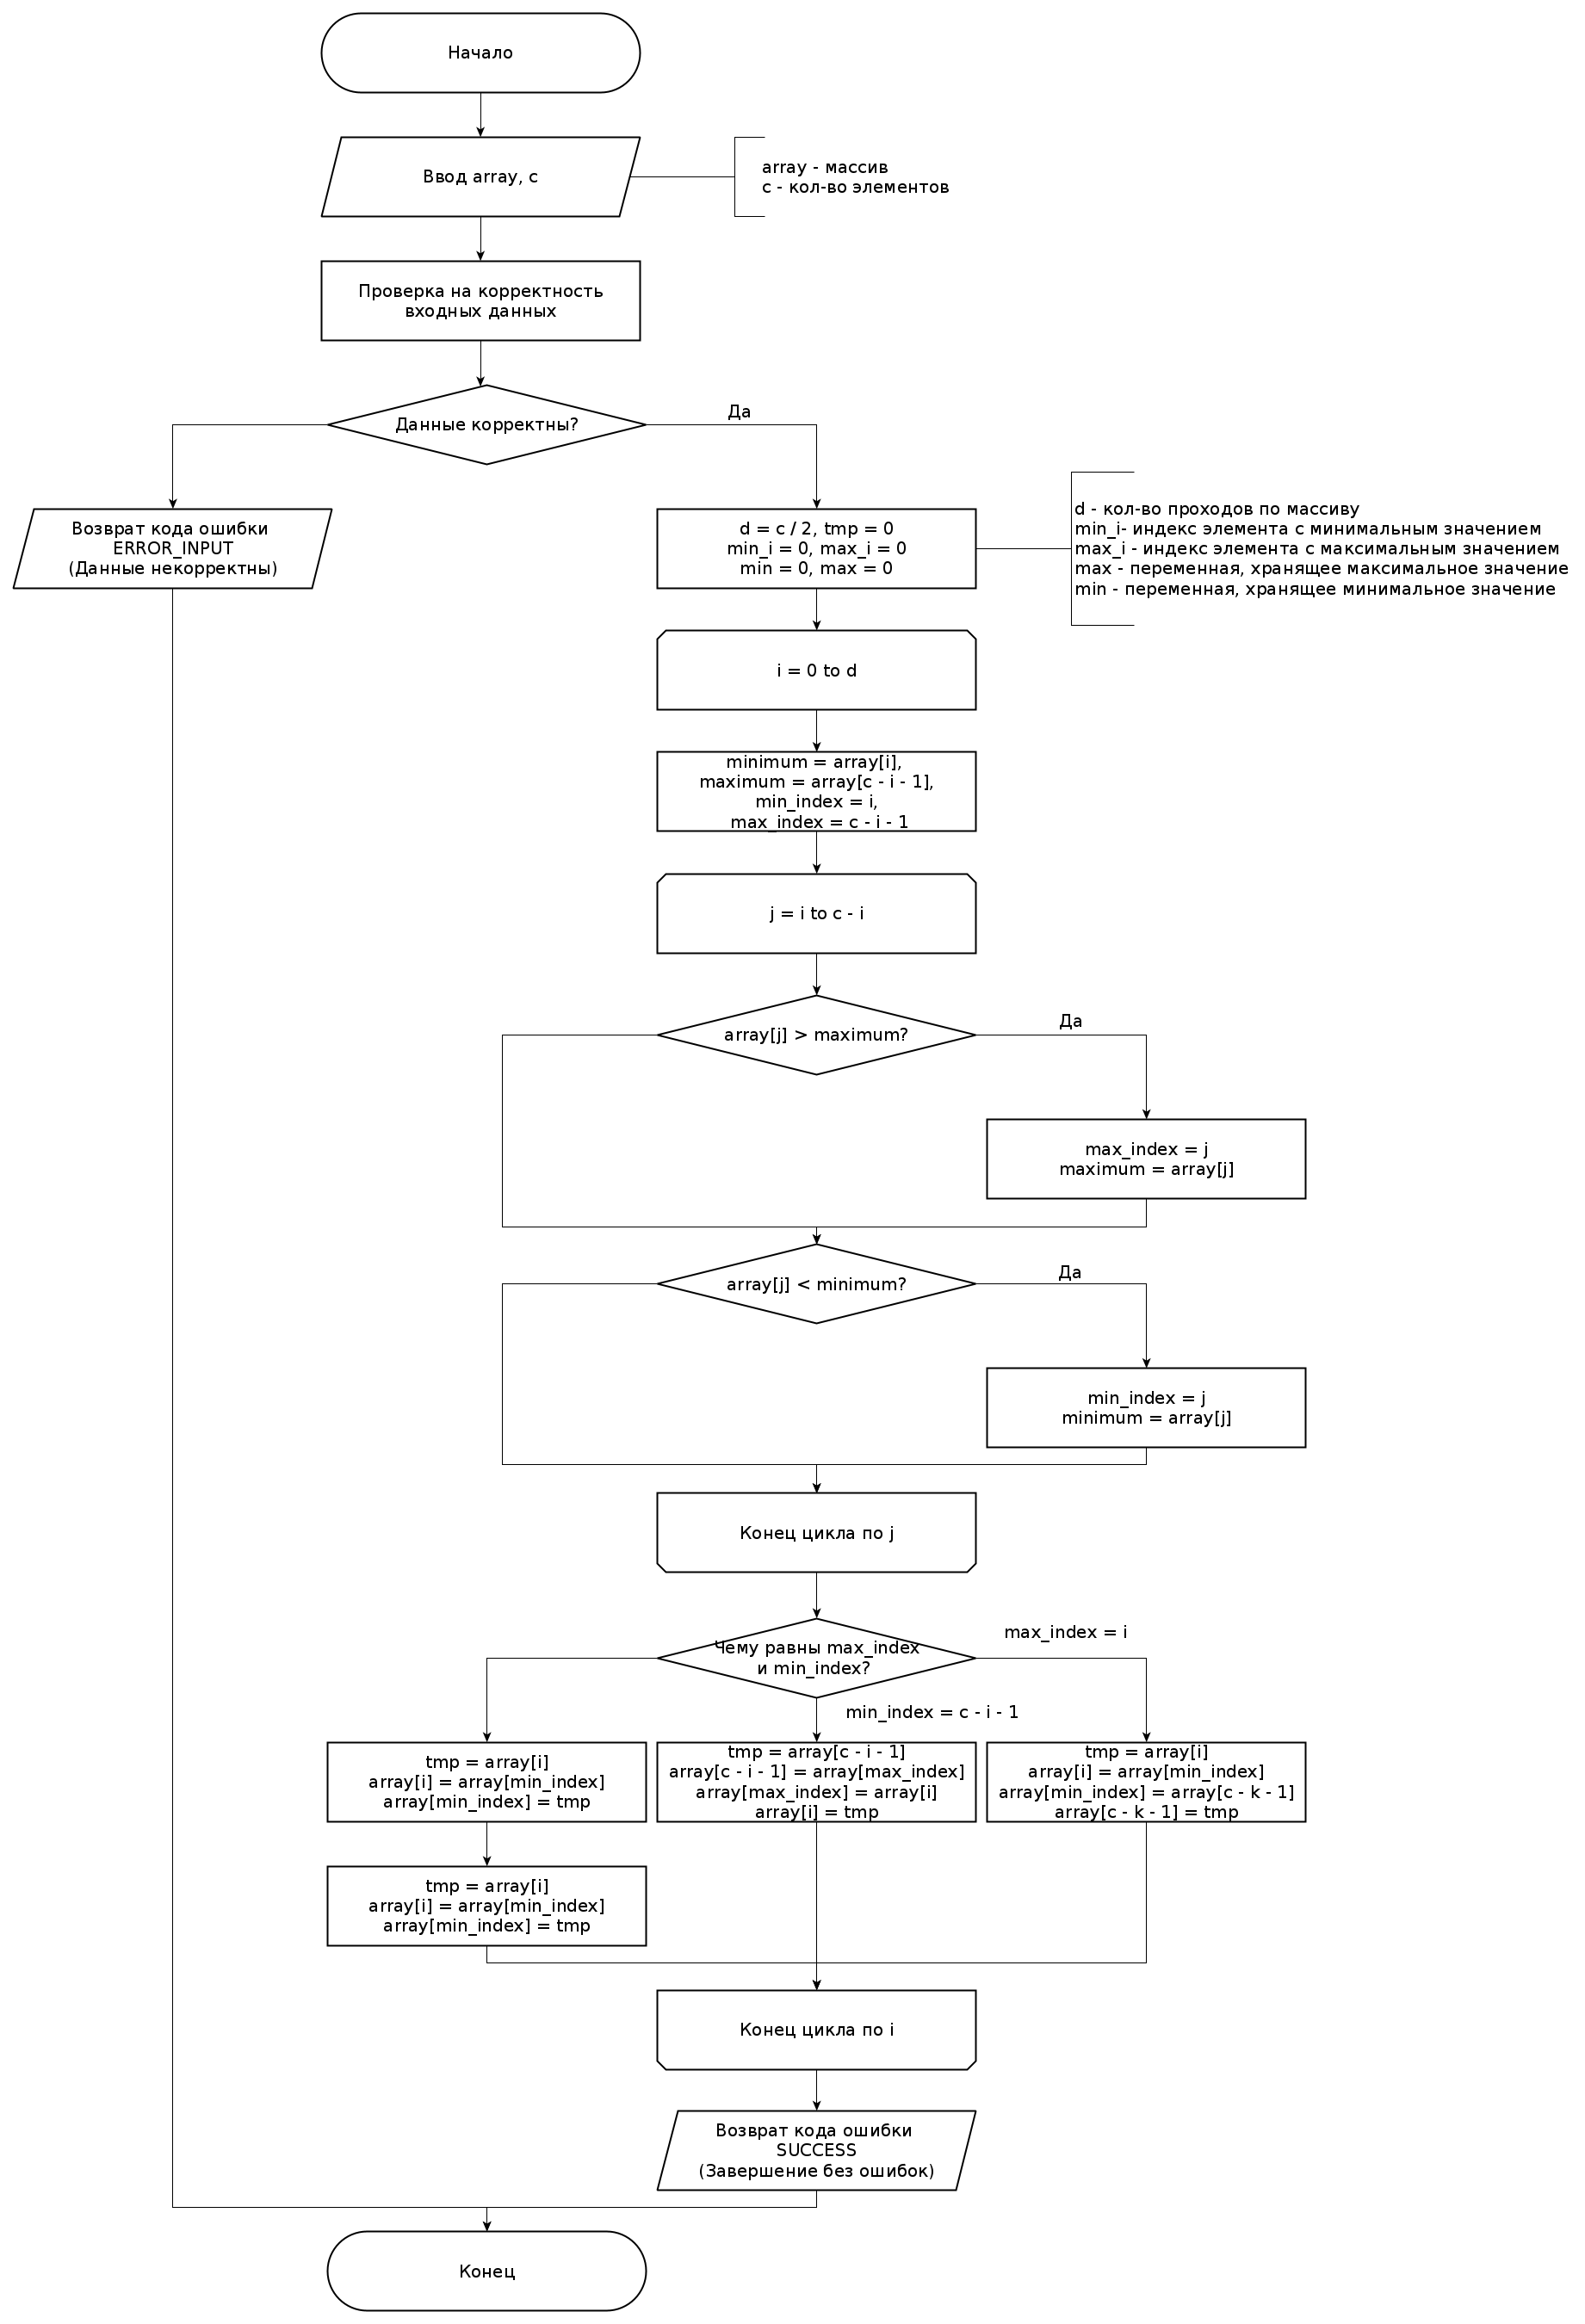
\includegraphics[scale=0.2]{sort_min_max.png}}
\caption{Схема алгоритма сортировки минимум/максимум}
\label{images:scheme2}
\end{figure}
\begin{figure}[p]
\center{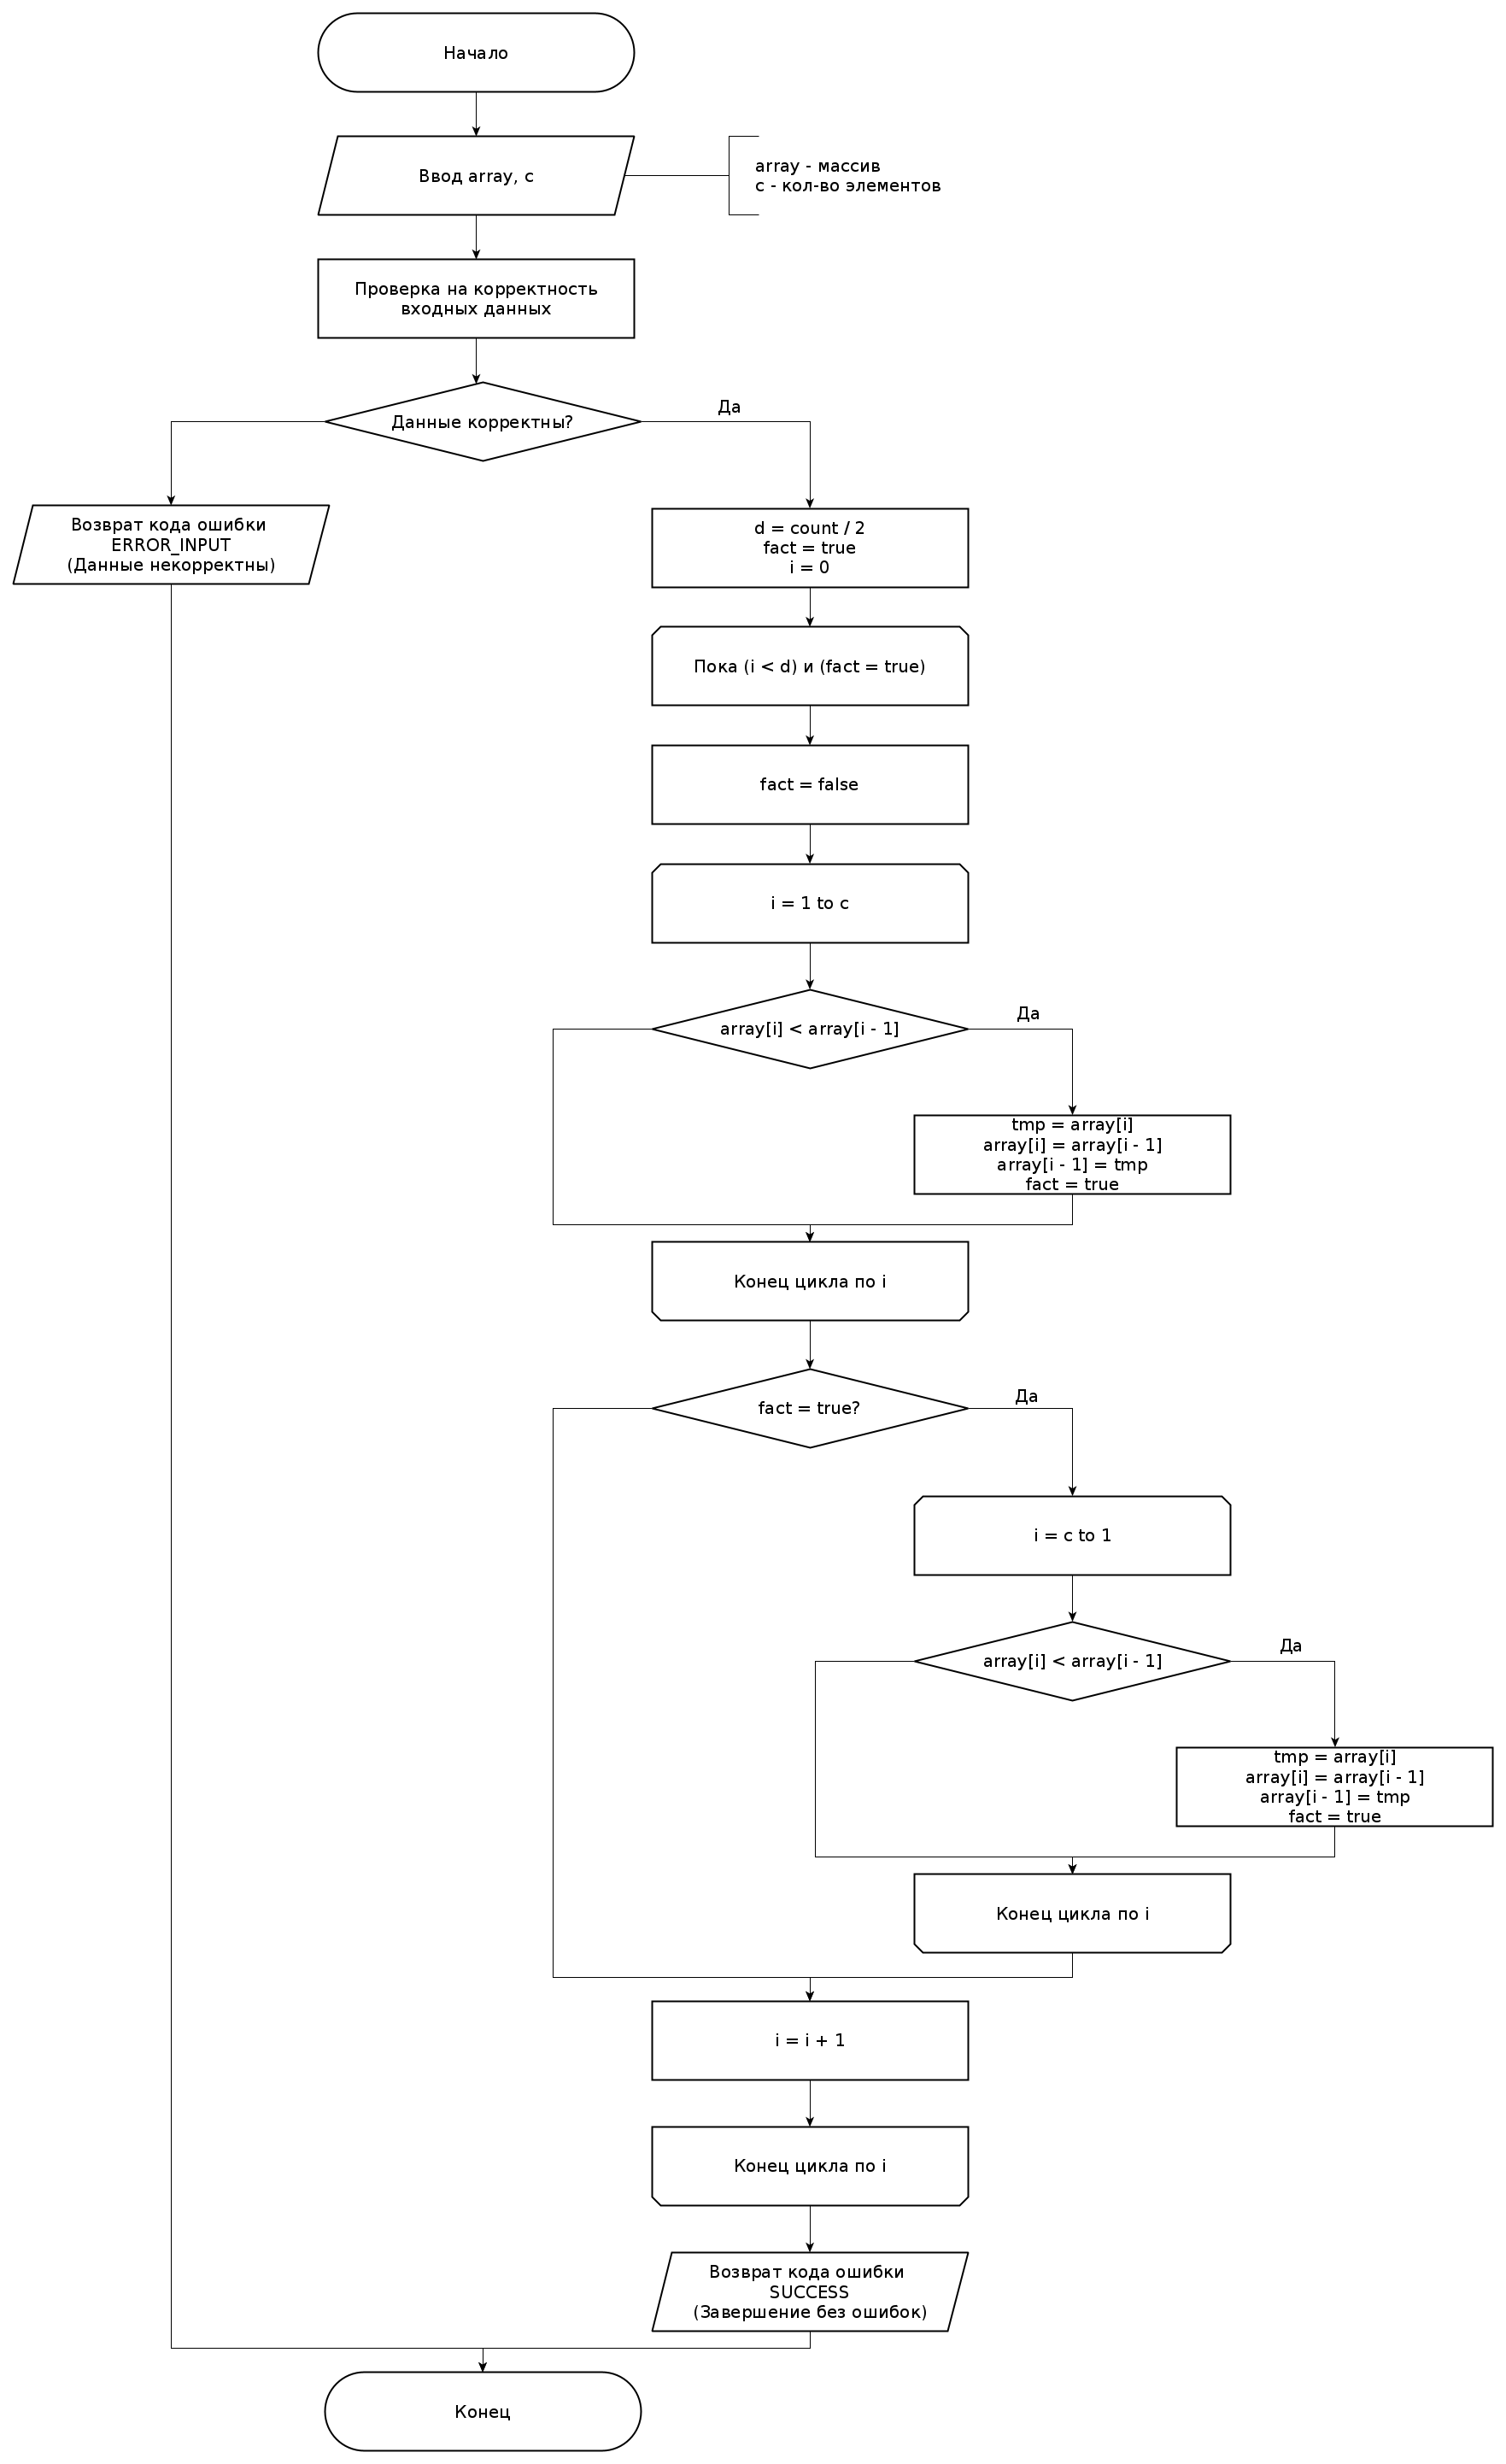
\includegraphics[scale=0.2]{sort_shaker.png}}
\caption{Схема алгоритма шейкерной сортировки}
\label{images:scheme3}
\end{figure}

\newpage
\subsection{Вывод}
На основе аналитических данных были разработаны требования к разрабатываемым лагоритм, а также приблизительные схемы работы алгоритмов.


\newpage
\section{ТЕХНОЛОГИЧЕСКАЯ ЧАСТЬ}
\subsection{Требования к программному обеспечению}

Программа должна работать на операционной системе Arch Linux. Программа должна содержать 2 режима:
\begin{itemize}
\item Пользовательский
\item Экспериментальный
\end{itemize}
В пользовательском режиме пользователь должен иметь возможность вводить строки и получать результат работы 3-х алгоритмов. В экспериментальном режиме засекается процессорное время работы каждого алгоритма, результаты записываются в отдельные файлы. Впоследствии данные из этих файлов можно вывести в виде графика.

\newpage
\subsection{Средства реализации}
Для реализации данных алгоритмов был выбран язык программирования С, компилятор gcc и некоторые функции из библиотеки glibc (memcpy, malloc и тд...). \\
Для вывода графиков использовался Python3 версии 3.7. В качестве библиотеки для отрисовки графиков была выбрана Matplotlib.

\newpage
\subsection{Листинг кода}
Ниже приведены реализации алгоритмов на С.\\
\lstdefinestyle{customc}{
  belowcaptionskip=1\baselineskip,
  breaklines=true,
  frame=L,
  xleftmargin=\parindent,
  language=C,
  showstringspaces=false,
  basicstyle=\footnotesize\ttfamily
}

\lstinputlisting[captionpos=b, caption=\label{listings:listing2}Сортировка пузырьком(\ref{images:scheme1}), style=customc]{listing2.c}
\newpage
\lstinputlisting[captionpos=b, caption=\label{listings:listing1}Сортировка минимум/максимум (двусторонняя сортировка выбором)(\ref{images:scheme2}), style=customc]{listing1.c}
\newpage
\lstinputlisting[captionpos=b, caption=\label{listings:listing3}Шейкерная сортировка(\ref{images:scheme3}), style=customc]{listing3.c}

\newpage
\subsection{Вывод}
Используя язык программирования C, в ходе практической работы были спроектированы и написаны реализации алгоритмов сортировки. Используя эти реализации были написаны 2 приложения: пользовательское приложение и приложение для подсчета времени выполнения этих алгоритмов.

\newpage
\section{ЭКСПЕРИМЕНТАЛЬНАЯ ЧАСТЬ}
\subsection{Характеристики аппаратного и программного обеспечения}
% Часть которую никогда нельзя менять
Тестирование приложения проводилось на машине со следующими характеристиками:\\
\begin{itemize}
\item Процессор Intel® Core™ i7-7700HQ;
\item Оперативная память 16 ГБ;
\item Операционная система - Arch Linux с рабочим окружением Gnome 3.
\end{itemize}

\newpage
\subsection{Примеры работы}
На Рис. ?, предсавленном ниже, демонстрируется работа приложения. Запуск приложения осуществляется из эмулятора терминала в Arch Linux. Во время работы приложение запрашивает у пользователя параметры массива и выводит результаты сортировки на экран.
\begin{figure}[h]
\center{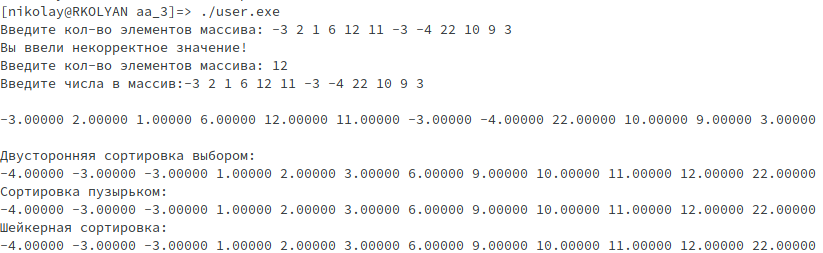
\includegraphics[scale=0.5]{example.png}}
\caption{Пример работы приложения}
\label{images:example}
\end{figure}

\newpage
\subsection{Результаты тестирования}
Ниже в таблице предоставлены результаты тестирования приложения.
Все результаты корректны и ссответствуют теоретическим результатам.
\begin{table}[h]
\caption{\label{tablice:tests}Результаты тестирования приложения}
\begin{center}
\begin{tabular}{|c|c|c|c|}
\hline
Массив & Реультат 1 & Результат 2 & Результат 3 \\
\hline
1 & 1 & 1 & 1 \\
\hline
1 2 3 & 1 2 3 & 1 2 3 & 1 2 3 \\
\hline
2 1 & 1 2 & 1 2 & 1 2 \\
\hline
2 1 3 & 1 2 3 & 1 2 3 & 1 2 3 \\
\hline
3 2 1 & 1 2 3 & 1 2 3 & 1 2 3 \\
\hline
4 3 2 1 & 1 2 3 4 & 1 2 3 4 & 1 2 3 4 \\
\hline
\end{tabular}
\end{center}
\end{table}

\newpage
\subsection{Постановка эксперимента по замеру времени}
Для вычисления процессорного времени работы алгоритмов использовалась функция clock(), объявленная в заголовочном файле time.h из библиотеки glibc. \\
Требования к программе, считающей время выполнения алгоритмов:
\begin{itemize}
\item Ввод пользователем таких параметров, как:
\begin{itemize}
\item Максимальный размер массива;
\item Кол-во итераций на каждый рассматриваемый случай (для высчитывания среднего значения времени);
\end{itemize}
\item Массивы генерируются со случайными числами;
\item Результаты вычислений должны сохранятся в текстовых файлах.
\end{itemize}

\newpage
\subsection{Сравнительный анализ на материале экспериментальных данных}
На Рис. \ref{images:graphics1},\ref{images:graphics2},\ref{images:graphics3} приведены графики зависимостей времени выполнения сортировок от размера массива. Единица измерения времени – временный такт процессора. \\

\begin{figure}[h]
\center{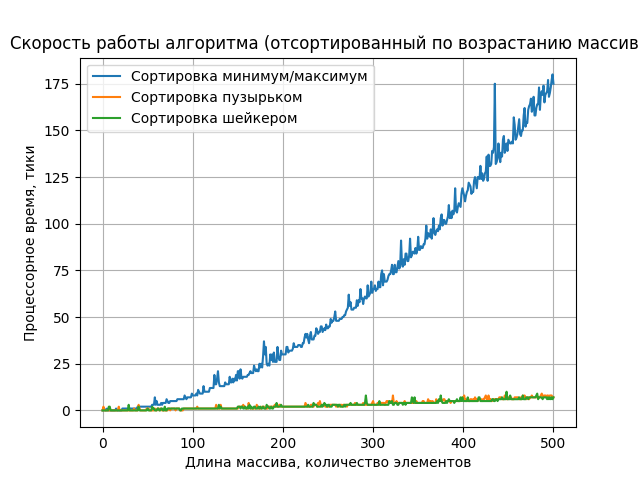
\includegraphics[scale=1]{graphics_sorted.png}}
\caption{График зависимости времени выполнения сортировок от размера массива}
\label{images:graphics1}
\end{figure}
\begin{figure}[H]
\center{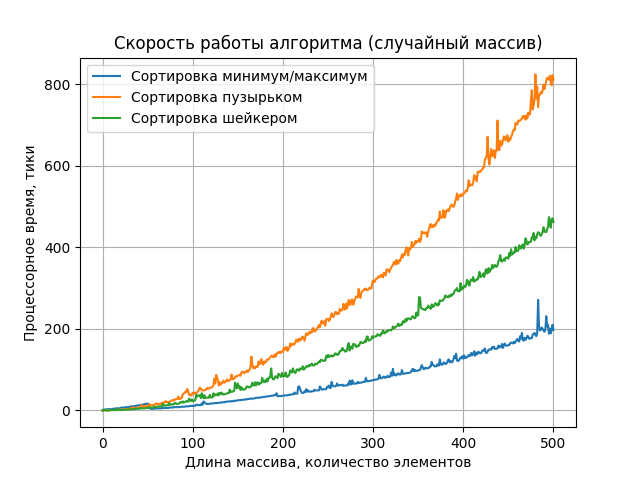
\includegraphics[scale=1]{graphics_random.png}}
\caption{График зависимости времени выполнения сортировок от размера массива}
\label{images:graphics2}
\end{figure}
\begin{figure}[H]
\center{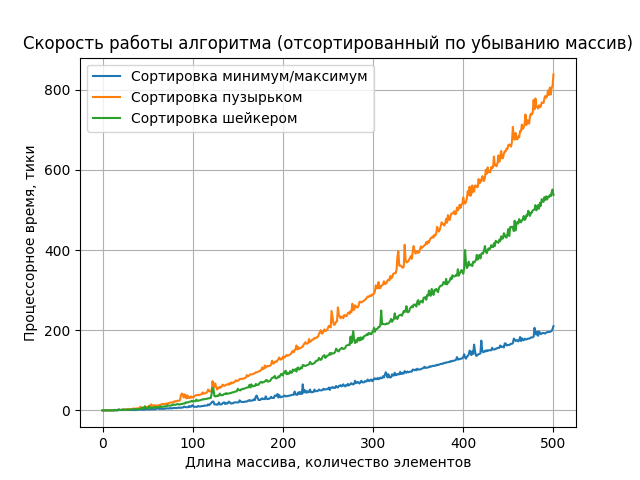
\includegraphics[scale=1]{graphics_unsorted.png}}
\caption{График зависимости времени выполнения сортировок от размера массива}
\label{images:graphics3}
\end{figure}

\newpage
\subsection{Оценка затрачиваемой памяти}
Размер памяти (в байтах) $M$, используемый во всех предоставленных алгоритмов сортировки можно вычислить по формуле:\\
\begin{equation}
M = N * t + S
\end{equation}
где:\\
$N$ - Кол-во элементов,\\
$t$ - размер типа данных в байтах(например, для integer - 4 байт, для double 8 байт),\\
$S$ - Память, выделяемая под вспомогательные элементы.\\

\newpage
\subsection{Вывод}
В результате исследования оценки времени выполнения можно сделать вывод, что сортировка пузырьком имеет самые худшие временные показатели. Сортировка методом поиска минимума и максимума самая быстрая и не зависит от расположения элементов. Для того, чтобы не наблюдалось случая, как представлено на графике[\ref{images:graphics1}], достаточно сделать вначале проверку на сортированость.

\newpage
\anonsection{ЗАКЛЮЧЕНИЕ}
Основное и единственное предназначение алгоритмов сортировок - упорядочивать данные. Везде где есть базы данных нужно так или иначе сортировать списки данных как для удобства пользователя, так и для индексации таблиц что бы быстро работал поиск. В библиотеке данные о книгах могут быть отсортированы по названию, по автору, по жанрам, по году издания. Тогда намного легче по картотеке или электронной базе найти интересующий экземпляр. 


\newpage
\anonsection{СПИСОК ИСТОЧНИКОВ}
\begin{itemize}
\item \label{site:wikipedia}https://ru.wikipedia.org/wiki/
\item \label{site:habr}https://habr.com/ru/post/422085/
\end{itemize}

\end{document}
